\documentclass[sigconf]{acmart}

\usepackage{booktabs} % For formal tables
\usepackage[vlined,linesnumbered,ruled,noend]{algorithm2e}     % algorithms
\usepackage[show]{chato-notes}
\usepackage{natbib}
\usepackage{tikz}
\usetikzlibrary{automata,arrows,positioning,calc}
\usepackage{lipsum}% http://ctan.org/pkg/lipsum
\usepackage{multicol}% http://ctan.org/pkg/multicols
\usepackage{float}
\usepackage{wrapfig}

%!TEX root = main.tex

% notations
\renewcommand{\vec}[1]{\ensuremath{\mathbf{#1}}} % vector
\newcommand{\matr}[1]{\ensuremath{\mathbf{#1}}} % matrix
\newcommand{\transpose}[1]{\ensuremath{\mathbf{#1}^\intercal}} % transpose

% Dot product notation
\makeatletter
\newcommand*\bigcdot{\mathpalette\bigcdot@{.5}}
\newcommand*\bigcdot@[2]{\mathbin{\vcenter{\hbox{\scalebox{#2}{$\m@th#1\bullet$}}}}}
\makeatother

% special terms
\newcommand{\markovchain}{{\it Markov Chain}}
\newcommand{\mdp}{{\it Markov Decision Process}}
\newcommand{\totalexpectedearnings}{{\it total expected earnings}}
\newcommand{\nominalproblem}{{\it nominal problem}}
\newcommand{\robustcontrolproblem}{{\it robust control problem}}
\newcommand{\epsilonsuboptimal}{\ensuremath{\epsilon}-\textit{suboptimal policy}}

%problems
\newcommand{\originalproblem}{{\textsc{MaxEarnings}}}
\newcommand{\robustproblem}{{\textsc{RobustEarnings}}}

% strategies
\newcommand{\naive}{{\textsc{Naive Strategy}}}
\newcommand{\relocation}{{\textsc{Relocation Strategy}}}
\newcommand{\flexible}{{\textsc{Flexible Schedule Strategy}}}
\newcommand{\relocationflexible}{{\textsc{Relocation with Flexible Schedule Strategy}}}
\newcommand{\earningsgoal}{{\textsc{Fixed Earnings Goal Strategy}}}

% actions
\newcommand{\getpassenger}{{\it Get Passenger}}
\newcommand{\gohome}{{\it Go Home}}
\newcommand{\relocate}{{\it Relocate}}

% symbols
\newcommand{\cityzones}{\ensuremath{\mathcal{X}}}
\newcommand{\countmatrix}{{\matr{C}}}
\newcommand{\rowcountmatrix}{{\mathbf{c}}}
\newcommand{\empiricaltransitionmatrix}{{\matr{F}}}
\newcommand{\truetransitionmatrix}{{\matr{P}}}
\newcommand{\rowtruetransitionmatrix}{{\mathbf{p}}}
\newcommand{\traveltimematrix}{{\matr{T}}}
\newcommand{\rewardsmatrix}{{\matr{R}}}
\newcommand{\homezone}{{\ensuremath{i_0}}}
\newcommand{\actionsset}{\ensuremath{\mathcal{A}}}
\newcommand{\policy}{\ensuremath{\pi}}
\newcommand{\policyspace}{\ensuremath{\Pi}}
\newcommand{\getpassengeraction}{\ensuremath{a_0}}
\newcommand{\gohomeaction}{\ensuremath{a_1}}
\newcommand{\relocateaction}{\ensuremath{a_2(j)}}
\newcommand{\actualaction}{\ensuremath{\hat{a}}}
\newcommand{\actuallocation}{\ensuremath{\hat{i}}}
\newcommand{\actualtime}{\ensuremath{\hat{t}}}
\newcommand{\earnings}{\ensuremath{\mathcal{E}}}
\newcommand{\betamax}{\ensuremath{\beta_{\textrm{max}}}}
\newcommand{\likelihoodregion}{\ensuremath{\mathcal{P}}}
\newcommand{\vmin}{\ensuremath{v_{\textrm{min}}}}
\newcommand{\vmax}{\ensuremath{v_{\textrm{max}}}}
\newcommand{\epsilonsuboptimalpolicy}{\ensuremath{{\pi}^{\epsilon}}}
\newcommand{\passengerarrivalrate}{\ensuremath{\lambda}}
\newcommand{\driverarrivalrate}{\ensuremath{\mu}}


% For action reward #1 is subscript (zone) #2 is superscript (time) #3 is action.
\newcommand{\actionearning}[3]{\ensuremath{E({#1},{#2},{#3})}}
\newcommand{\cumulativeearning}[2]{\ensuremath{v_{#1}^{#2}}}
\newcommand{\inducedearningvector}[3]{\ensuremath{\mathbf{v}_{#1}^{#2}({#3})}}


\DeclareMathOperator*{\argmin}{arg\,min}
\DeclareMathOperator*{\argmax}{arg\,max}

\newcommand{\etal}{\emph{et al.}}

%formating
\newcommand{\spara}[1]{\smallskip\noindent{\bf{#1}}}
\newcommand{\mpara}[1]{\medskip\noindent{\bf{#1}}}
\newcommand{\bpara}[1]{\bigskip\noindent{\bf{#1}}}

\newcommand{\squishlist}{\begin{list}{$\bullet$}
  { \setlength{\itemsep}{0pt}
     \setlength{\parsep}{3pt}
     \setlength{\topsep}{3pt}
     \setlength{\partopsep}{0pt}
     \setlength{\leftmargin}{1.5em}
     \setlength{\labelwidth}{1em}
     \setlength{\labelsep}{0.5em} } }
\newcommand{\squishend}{
  \end{list}  }
  
  \newtheorem{problem}{Problem}



% Copyright
% \setcopyright{none}
% \setcopyright{acmcopyright}
% \setcopyright{acmlicensed}
% \setcopyright{rightsretained}
% \setcopyright{usgov}
% \setcopyright{usgovmixed}
% \setcopyright{cagov}
% \setcopyright{cagovmixed}


% DOI
% \acmDOI{10.475/123_4}

% ISBN
% \acmISBN{123-4567-24-567/08/06}

%Conference
% \acmConference[SHORTNAME'17]{ACM Long Conference Name conference}{July 1997}{City, State, Country} 
% \acmYear{2017}
% \copyrightyear{2017}

% \acmPrice{15.00}


\begin{document}
\title{Putting Data in the Driver's Seat:\\
Optimizing Earnings for On-Demand Ridesharing}
% \titlenote{Produces the permission block, and copyright information}
% \subtitle{Extended Abstract}


%\author{Harshal A. Chaudhari}
%\affiliation{%
%  \institution{Boston University}
%}
%\email{harshal@cs.bu.edu}
%
%\author{John W. Byers}
%\affiliation{%
%  \institution{Boston University}
%}
%\email{byers@cs.bu.edu}
%
%\author{Evimaria Terzi}
%\affiliation{%
%  \institution{Boston University}
%}
%\email{evimaria@cs.bu.edu}

% The default list of authors is too long for headers}
% \renewcommand{\shortauthors}{F. Lastname et al.}

%
% The code below should be generated by the tool at
% http://dl.acm.org/ccs.cfm
% Please copy and paste the code instead of the example below. 
%
% \begin{CCSXML}
% <ccs2012>
%  <concept>
%   <concept_id>10010520.10010553.10010562</concept_id>
%   <concept_desc>Computer systems organization~Embedded systems</concept_desc>
%   <concept_significance>500</concept_significance>
%  </concept>
%  <concept>
%   <concept_id>10010520.10010575.10010755</concept_id>
%   <concept_desc>Computer systems organization~Redundancy</concept_desc>
%   <concept_significance>300</concept_significance>
%  </concept>
%  <concept>
%   <concept_id>10010520.10010553.10010554</concept_id>
%   <concept_desc>Computer systems organization~Robotics</concept_desc>
%   <concept_significance>100</concept_significance>
%  </concept>
%  <concept>
%   <concept_id>10003033.10003083.10003095</concept_id>
%   <concept_desc>Networks~Network reliability</concept_desc>
%   <concept_significance>100</concept_significance>
%  </concept>
% </ccs2012>  
% \end{CCSXML}
% 
% \ccsdesc[500]{Computer systems organization~Embedded systems}
% \ccsdesc[300]{Computer systems organization~Redundancy}
% \ccsdesc{Computer systems organization~Robotics}
% \ccsdesc[100]{Networks~Network reliability}

% We no longer use \terms command
%\terms{Theory}

%!TEX root = main.tex

\begin{abstract}
On-demand ride-hailing platforms like Uber and Lyft are helping reshape urban transportation, by enabling car owners to become drivers for hire with minimal overhead. Although there are many studies that consider ride-hailing platforms holistically, e.g., from the perspective of supply and demand equilibria, little emphasis has been placed on optimization for the individual, self-interested drivers that currently comprise these fleets. While some individuals drive opportunistically either as their schedule allows or on a fixed schedule, we show that strategic behavior regarding when and where to drive can substantially increase driver income. In this paper, we formalize the problem of devising a driver strategy to maximize expected earnings, describe a series of dynamic programming algorithms to solve these problems under different sets of modeled actions available to the drivers, and exemplify the models and methods on a large scale simulation of driving for Uber in NYC. In our experiments, we use a newly-collected dataset that combines the NYC taxi rides dataset along with Uber API data, to build time-varying traffic and payout matrices for a representative six-month time period in greater NYC. From this input, we can reason about prospective itineraries and payoffs. Moreover, the framework enables us to rigorously reason about and analyze the sensitivity of our results to perturbations in the input data. Among our main findings is that repositioning throughout the day is key to maximizing driver earnings, whereas `chasing surge' is typically misguided and sometimes a costly move.
\end{abstract}


% \keywords{ACM proceedings}

\maketitle
%%%!TEX root = main.tex
  [JB: this does not go here]
%!TEX root = main.tex

\section{Introduction}
\label{sec:introduction}

The proliferation of on-demand ride-hailing platforms like Lyft and Uber
  has begun to fundamentally change the nature of urban transit. 
In the last two years alone, the number of daily trips using ride-hailing 
  platforms like Uber and Lyft in NYC has grown five-fold, 
  to about 350,000 trips per day. 
Today, over 65,000 drivers drive on the streets of NYC as Uber or Lyft drivers.
The explosive growth of these ride-hailing platforms has motivated a wide
  array of questions for academic research at the intersection of computer
  science and economics, ranging from the design of effective pricing mechanisms, 
  to equilibrium analysis, to the design of reputation management systems for 
  drivers, to algorithms for matching drivers with 
  customers, as we discuss in our related work section.
%%~\cite{banerjee2015pricing,ozkan2016dynamic}.

While these studies consider the study of ride-hailing platforms holistically, 
   little work has been done on optimizing strategies for individual drivers. 
Nevertheless, the challenge of how to maximize one's individual earnings as a driver for a 
ride-hailing platform like Uber or Lyft is a pressing question that millions of micro-entrepreneurs 
across the world now face.  Anecdotally, many drivers spend a great deal of time 
strategizing about where and when to drive.  However, drivers today are 
self-taught, using heuristics of their own devising or learning from one another, 
and employ relatively simple analytics dashboards such as SherpaShare.
Indeed, rumors suggest that some drivers even collude in attempts to induce spikes in surge prices that they can then exploit.
But in terms of concrete guidance, to date, there are only articles in the
  popular press and on blogs that offer (often contradictory) advice to ride-hailing drivers 
  how to maximize their earnings~\cite{dont,tips,sherpashareNYT}.

In this paper, we formalize the problem of devising a driver strategy to maximize expected 
 earnings and describe a series of dynamic programming algorithms to solve this problem
 under different sets of modeled actions available to the drivers. 
Our strategies take as input a detailed model of city-level data that constitutes a 
  fine-grained weekly projection of forecasted demand for rides, comprising 
  predicted spatiotemporal distributions of source-destination pairs, driver payments,
  transit times, and surge multipliers. 
The optimization framework we propose not only produces contingency plans in the form of
  highly optimized driving schedules and real-time in-course corrections to drivers, but 
  also enables us to rigorously reason about and analyze the sensitivity of our output 
  results to perturbations in the input data.  
Thus, we can justify the proposed strategies even under an uncertainty level in the
  collected data and the data model itself.
  
We then exemplify our  results with a large-scale simulation of driving for Uber in NYC. 
For this simulation, we assemble a new dataset that uses both the publicly available NYC taxi rides 
dataset~\footnote{\url{http://www.nyc.gov/html/tlc/html/about/trip_record_data.shtml}} as well as calls to the Uber API.
From the former, we obtain information about over 200,000 taxi rides that occurred between different NYC zones. 
From the latter, we obtain representative pricing and traffic-time information for those trips, were they to reoccur on Uber.
From this newly-collected dataset, we construct a mathematical model to produce input to our algorithms. 
However, we view the dataset, which we plan to release, to be of independent interest that could subsequently 
be used for a multitude of other studies.

Our experiments with our methods on this dataset demonstrate the following findings:
being strategic about the areas they focus on picking up riders and the times they work, 
can significantly increase a driver's income, sometimes by
as much as 1.75x, when compared to a naive optimization strategy.
Moreover, we show that a pronounced difference between the earnings obtained by the 
two strategies holds even when there is a large uncertainty in the input data. 
We argue that our results are therefore not purely an artifact of the NYC dataset we employ, 
  but also that they have high potential to generalize well.
Finally, our experiments show that naively chasing surging prices does not typically lead 
  to significant earnings gains, but it can even introduce large opportunity costs, as drivers
  waste time driving to subsiding surges. 

%!TEX root = main.tex

\section{Related Work}
\label{sec:related_work}

To the best of our knowledge, we are the first to formally address the problem of optimizing
the driver's strategy in ridesharing platforms like Lyft and Uber. 
Interestingly, there have been recent articles in the popular press as well as blogposts on 
offering (often contradictory) advice to ridesharing drivers how to maximize earnings, mostly via chasing surge~\cite{dont,tips}.

To the best of our knowledge, the only relevant existing technical work 
studies other aspects of ridesharing platforms like Lyft and Uber. 
Also related can be considered existing work on optimization problems related to taxi routes. We discuss existing works along these lines next.


\spara{Studies of ridesharing platforms:}
Recent work has investigated the supply-side effects of specific incentives that Uber and Lyft provide to drivers, notably the impact of surge pricing~\cite{slaves}.  For example, Chen and Sheldon}~\cite{chen2016dynamic} show 
a causal relationship that drivers on Uber respond to surges by driving more during high surge times,  differentiating from previous work that suggests taxi drivers primarily focus on achieving earnings goals~\cite{camerer1997labor}. 
Other work has viewed ridesharing platforms more holistically, at a macro level.
Work by Chen {\etal}}~\cite{chen2015peeking} measured many facets of Uber in NYC, including the prevalence and extent 
  of surge pricing.
Work by Hall {\etal}~\cite{hall2016analysis} showed that drivers were attracted to Uber platform due to flexibility it offers, 
and the level of compensation, but that earnings per hour do not vary much with number of hours worked. 
All these studies perform an {\em a posteriori} analysis of the data
and they do not focus on devising specific recommendations for drivers as we do.


 In another line of work on these platforms, Banerjee {\etal}~\cite{banerjee2015pricing} studied complex dynamic
pricing strategies for ridesharing platforms such as Lyft using a queuing-theoretic economic model. 
They show that dynamic pricing is robust to changes in system parameters, even if it does not 
  achieve higher performance than static pricing.  
More recently, Ozkan and Ward\cite{ozkan2016dynamic} looked at strategic matching between supply (individual drivers) 
  and demand (requested rides) for Uber and Lyft.
 hey showed that matching based on parameters like driver and customer arrival rates, 
  willingness of customers to wait and time-variance can achieve better performance than naively matching 
  passengers with the closest driver. 
Although these works build interesting models for ridesharing economies, they are
 orthogonal to ours as they take a more holistic view of such economies, while we choose to focus 
 on earnings of individual, self-interested drivers.




\spara{Optimization problems for taxi fleets:}
A considerable body of related work has focused on the optimization of taxi fleets, for
example building economic network models to describe demand and supply equilibria of taxi 
services under various tariff structures, fleet size regulations and other policy
alternatives~\cite{bailey1987simulation,yang2002demand}.  More recent work seeks to 
maximize social welfare by optimizing allocation of taxi market resources~\cite{shi2016optimization}.
Another direction relates to route optimization by a centralized administrator, e.g., in
the context of online and offline taxi dispatching services~\cite{maciejewski2013simulation,nunes2011taxi} 
and in the case of maximizing occupancy and minimizing travel times (by minimizing passenger detours) 
in a shared-ride setting~\cite{jung2013design}.
Other work has studied the supply side of the driving market from the viewpoint of behavioral economics.
A seminal paper by ~\cite{camerer1997labor} studied cabdrivers and found that  (1) `inexperienced' 
cabdrivers make labor supply decisions ``one day at a time'' instead of substituting labor and leisure 
across multiple days, and  (2) set a loose daily income target and quit working once they reach that 
target.  
Although related, all these works do not focus on the design of a specific gain-optimizing
strategy for drivers, as we do.

\begin{comment}

\textbf{Works on general taxi cabs:}

2. \cite{yang1998network} - first in the series of works modeling taxi utilization and movement to find that higher utilization leads to longer waiting times for customers.

3. \cite{wong2001modeling} - second paper, extends previous paper to incorporate effects of congestion and customer demand elasticity. 

4. \cite{yang2002demand} - third paper, uses network model to describe demand and supply equilibrium of taxi services under fare structure and fleet size regulation in competitive / monopoly market.

5. \cite{bailey1987simulation} - directed at understanding the dynamic interaction between demand, service rates and policy alternatives. Finds that customer waiting time is insensitive to changes in demand, but highly sensitive to changes in taxi fleet size.

6. \cite{qin2017mining} - explore the factors affecting driver incomes with quantitative estimates using GPS traces of over 167 million trips in Shanghai.

7. \cite{rong2016rich} - MDP to increase the revenue per unit time of taxi drivers. They study the relocate action from our strategy.

\textbf{Works on taxi routing:}

8. \cite{maciejewski2013simulation} - optimizes taxi routing by generating demand and congested network simulation. Defines online and offline taxi dispatching strategies and evaluate them. `No-scheduling' strategy works well under low demand but deteriorates under heavy load.

9. \cite{nunes2011taxi} - formulates a TSP problem to find best route for a taxi company to satisfy demand.

\textbf{Works on ride-sharing:}

10. \cite{agatz2012optimization} - outline optimization challenges in developing technology to support ride-sharing services. Survey of operations research papers in the domain.

11. \cite{santos2013dynamic} - Prove that problem of maximizing shared trips within a fixed time window to minimize shared expenses is NP-Hard and a propose heuristic solution.

12. \cite{jung2013design} - Simulated Annealing algorithm to maximize occupancy and minimize travel times (by minimizing passenger detours) in shared-ride concept.

\textbf{Works on ride-sharing vehicle routing:}

13. \cite{lin2012research} - simulated annealing algorithm to optimize routing of ride-sharing taxi to minimize operating costs while maximizing customer satisfaction.

\textbf{Strategic behavior:}

14. \cite{shi2016optimization} - maximizes social welfare and optimizes allocation of taxi market resources. Also analyzes strategic behavior of passengers who may join or drop out of system based on their social welfare threshold.

\textbf{Uber related works:}

15. \cite{hall2016analysis} - Drivers attracted to Uber platform due to flexibility it offers, level of compensation, earnings per hour do not vary much with number of hours worked. 

16. \cite{chen2016dynamic} - Show a causal relationship that drivers on Uber respond to `surges' by driving more during high surge times, in contrast to \cite{camerer1997labor} which says that drivers driver until they achieve earnings goals.

17. \cite{banerjee2015pricing} - Study complex dynamic pricing strategies for ride-sharing platforms (Lyft) using a queuing-theoretic economic model. They show the dynamic pricing is robust to changes in system parameters, even if it does not achieve higher performance than static pricing. 

18. \cite{ozkan2016dynamic} - Strategic matching between Uber or Lyft's supply and demand. Matching based on parameters like customer/driver arrival rates, willingness of customers to wait and time-variance can achieve better performance than naively matching passenger with closest driver.

\textbf{Media and Press articles:}


 

%%3. 
\end{comment}

%!TEX root = main.tex

\section{Problem setup}
\label{sec:problem_setup}

In this section, we describe the basics of our problem setup and provide the necessary notation.

\iffalse
\subsection{Notation}
\label{sec:notation}

Vectors are denoted with lowercase bold letters (e.g., $\vec{a} = [a(i)]$) and matrices are denoted with uppercase bold letters (e.g., $\matr{A} = [a(i,j)]$). The notation $\vec{1}$ refers to the vector of ones, with size dependent on the context. The short form notation $\vec{A_i}$ refers to the $i$-th row vector of the matrix $\matr{A}$. Let $\Theta_n$ be a set of $n \times n$ right-stochastic transition matrices (non-negative matrices with rows that sum to one). A probability simplex in $\mathbb{R}^n$ is denoted by $\Delta_n = \{\vec{p} \in \mathbb{R}^n_+ : \transpose{p} \vec{1} = 1 \}$.
\fi

\subsection{Modeling the city}

Throughout the paper, we will assume that a city is divided into non-overlapping set of zones denoted by \cityzones. 
We represent a city in the form of a weighted directed graph $G=(\cityzones, E)$ with 
$|\cityzones| = n$ and $|E| = {n \choose 2}$ edges, an edge between each pair of nodes. 
Some of the attributes of a city (over a fixed time interval) are as follows:

%\subsubsection{\sc{EmpiricalTransitionMatrix} (\empiricaltransitionmatrix)}

\spara{Count matrix (\countmatrix)}: 
Every edge $e(i\rightarrow j) \in E$ is associated with an
integer-valued weight $c(i,j)$ that denotes the number of requests
at zone $i$ that had node $j$ as their destination.

\spara{Empirical transition matrix (\empiricaltransitionmatrix)}:
The count matrix gives rise to the transition matrix {\empiricaltransitionmatrix}.
The entries of {\empiricaltransitionmatrix} correspond to probabilites and thus
$f(i,j) \in [0,1]$ such that
$\sum_{j \in \cityzones} f(i,j) = 1$, $\forall i \in \cityzones$.

Therefore, the weights give rise to a {\markovchain} with a transition matrix {\empiricaltransitionmatrix} -- 
where each entry $f(i,j)$ 
denotes the empirically observed probability of a passenger in zone $i$
traveling to zone $j$. 
As a special case, 
$f(i,i)$ denotes the probability of not finding a passenger in zone $i$. 
%The empirical transition matrix {\empiricaltransitionmatrix}
%changes throughout the day. Hence, we use $\empiricaltransitionmatrix^t$ to denote the matrix at time $t$.

%\subsubsection{\sc{TravelTimeMatrix} (\traveltimematrix)}

\spara{Travel time matrix (\traveltimematrix)}:
Every edge $e(i\rightarrow j) \in E$ is also associated with a positive valued weight $\tau(i,j) > 0$ 
denoting the travel time duration for a ride from zone $i$ to zone $j$. 
These weights give us a travel time matrix {\traveltimematrix} with entries $\tau(i,j)$. 
%Just like {\empiricaltransitionmatrix},  travel time matrix also evolves throughout the day. 
%Hence, we use $\traveltimematrix^t$ to denote the matrix at time $t$.

%\subsubsection{\sc{RewardsMatrix} (\rewardsmatrix)}

\spara{Rewards matrix (\rewardsmatrix)}:
Every edge $e(i \rightarrow j) \in E$ is also associated with a real valued reward $r(i,j)$ denoting
the net reward for a driver delivering a passenger from zone $i$ to zone $j$. The net rewards include the driver's
share of earnings from a passenger minus the sundry costs like gas, vehicle depreciation, etc.  Since these
earnings and costs vary with mileage and transit time, each entry in the rewards matrix $\rewardsmatrix$ 
is of the form $r(i,j)$ = earnings$(i,j)$ - cost$(i,j)$.
%Following our earlier convention, rewards matrix at time $t$ is denoted by $\rewardsmatrix^t$.

Note that all the above matrices, {\countmatrix}, {\empiricaltransitionmatrix}, {\traveltimematrix} and {\rewardsmatrix}, are time dependent, i.e., their entries change throughout the day. Therefore, at any point in time $t$, the instantiations of these matrices
are different. We denote those instantiations by $\countmatrix^t$, $\empiricaltransitionmatrix^t$, $\traveltimematrix^t$ and $\rewardsmatrix^t$ respectively.
For clarity of exposition we will ignore the time-dependent aspect of the model in what follows.


\subsection{Modeling the driver}
Throughout the paper, we will assume that 
each driver comes with a 
maximum budget of $B$ time units
he is willing to work. During these time units the driver 
 can pick
up passenger rides. Depending on the specific setting, the driver can
work $B$ time units consecutively or split them 
over a finite horizon of $N$ time units. Obviously, $N \geq B$. 
As an example, a driver seeking to optimize a 40 hour work week over
a 7 day week shall have $B=40$ hours and $N=168$ hours.

%\subsubsection{\sc{HomeZone} (\homezone)}

\spara{Home zone (\homezone)}: 
Each driver has a unique home zone denoted by $i_0 \in \cityzones$. 
We always assume that the driver starts from his home zone and returns to it
at the end of each of his shifts.
%\subsubsection{\sc{DriverActions} (\actionsset)}

\spara{Driver actions (\actionsset)}: 
Whenever faced with making a decision regarding next decision during a driving strategy, a driver has $n+2$ possible actions he can take: 
%\begin{itemize}
\squishlist
	\item {\getpassenger} (\getpassengeraction): Wait for a passenger in the current zone. 
	\item {\gohome} (\gohomeaction): Log out of the on-demand ride service, relocate to the home zone (if needed) 
  and stop working.   This action does not consume the driver's budget.
	\item {\relocate} (\relocateaction): Relocate to city zone $j$.  This action consumes the driver's budget.
%\end{itemize}
\squishend

%\subsubsection{\sc{DriverPolicy} (\policy)}

\spara{Driver policy (\policy)}:
A driver policy is an ordered set of time and location dependent actions taken by a driver at different steps of the strategy. As the total number of actions taken by a driver while exhausting the budget $B$ depends on the actual actions, the length
of a driver policy {\policy} varies. 

Each time and location dependent action $\mathbf{a}$ in the {\policy} can be expressed in form of a 3-tuple -- $(\actualaction, \actuallocation, \actualtime)$
where $\actualaction \in \actionsset$ refers to actual action, $\actuallocation \in \cityzones$ is the zone at which action was taken and $\actualtime \leq N$ is the 
time at which the action was taken.

% A policy of length $L$, $\policy_L = (\mathbf{a}^1, \cdots, \mathbf{a}^L)$, induces
% three ordered sets of length $L$ each.

% \begin{itemize}
% 	\item \textit{Action Trajectory} : An ordered set of actions taken by driver following the policy, denoted by \actiontrajectory{\policy_L}.
% 	\item \textit{Location Trajectory} : An ordered set of nodes at which the driver takes each of the actions from \actiontrajectory{\policy_L}, denoted by \locationtrajectory{\policy_L}.
% 	\item \textit{Time Trajectory} : An ordered set of times at which the driver takes each of the actions from \actiontrajectory{\policy_L}, denoted by \timetrajectory{\policy_L}.
% \end{itemize}

Furthermore, for a policy of length $L$, the corresponding policy space can be denoted by
$\policyspace_L = \actionsset^{nL}$. The set of all possible policies is $\policyspace = \{\policyspace_1, \cdots, \policyspace_N\}$, as the maximum length of a policy can be $N$.


\subsection{Computing driver earnings}
In this section, we describe the computation of the expected earnings of a driver
who at a specific time $t$ is in zone $i$ and takes action $a$. We denote this by 
$\actionearning{i}{t}{a}$ and depending on the action $a$ it is computed as follows.

\squishlist
	\item For action {\getpassengeraction} ({\getpassenger}), taken inside zone $i$ at time $t$, the action earnings function
	is calculated as an expectation over possible rides,
	\begin{equation}\label{eq:a0}
	\actionearning{i}{t}{a_0} = \empiricaltransitionmatrix_{i}\bigcdot \rewardsmatrix_{i}
	\end{equation}
	where $\empiricaltransitionmatrix_{i}$ and $\rewardsmatrix_{i}$ denote the $i$-th rows of $\empiricaltransitionmatrix$ and $\rewardsmatrix$ respectively. 
	
	\item For action {\gohomeaction} ({\gohome}), taken inside zone $i$ at time $t$, the action earnings function is simply
	\begin{equation}\label{eq:a1}
	\actionearning{i}{t}{a_1} = - cost(i,\homezone)
	\end{equation}
	where we incur a negative reward due to the absence of a paying customer. 

	\item Action {\relocateaction} ({\relocate}), taken inside zone $i$ at time $t$, 
	takes the driver to zone $j \neq i$. Therefore, the action earnings function is 
	\begin{equation}\label{eq:a2}
	\actionearning{i}{t}{a_2(j)} = - cost(i,j)
	\end{equation}
	where the driver again incurs a negative reward due to the absence of a paying customer. 
%\end{itemize}
\squishend

%\subsubsection{\sc{CumulativeEarning}}
\iffalse
\spara{\sc{CumulativeEarning}}:
Cumulative Earning is a function of zone and time. Let {\cumulativeearning{i}{t,b}} denote the total expected future earnings of a driver
while inside zone $i$ at time $t$ with $b$ budget units consumed. Using this definition, total expected earnings of a driver can be expressed
as {\cumulativeearning{\homezone}{N,B}}.

%\subsubsection{\sc{InducedEarningVector}}
\spara{\sc{InducedEarningVector}}:
If a driver at zone $i$ at time $t$ with $b$ budget units consumed takes a passenger ride to zone $j$, the rides end at time 
$t' = t + \tau^t(i,j)$ with budget $b' = b + \tau^t(i,j)$ consumed. The \textsc{CumulativeEarning} of the driver in zone $j$ at time $t'$ with $b'$
budget units consumed is {\cumulativeearning{j}{t',b'}}. Let us denote using {\inducedearningvector{i}{t,b}{\getpassengeraction}} the vector of such
cumulative earnings across different zones $j$ induced when a driver takes an action {\getpassengeraction} and call it an 
\textsc{InducedEarningVector}. Instead of a vector of cumulative earnings, {\gohome} action induces a single value i.e., {\cumulativeearning{\homezone}{t',b}}. 
As the driver has logged out of system, the consumed budget units $b$ remained unchanged. {\relocate} action induces a single value of cumulative earnings per destination zone $j$, {\cumulativeearning{j}{t',b'}}. 
Using this formulation, for each of the driver actions, we can recursively express \textsc{CumulativeEarning} as follows,
\begin{itemize}
	\item {\getpassenger} : For {\getpassengeraction} taken inside zone $i$ at time $t$ with $b$ budget units consumed,
	\begin{eqnarray}
	\cumulativeearning{i}{t,b} &=& \actionearning{i}{t}{\getpassengeraction} + \empiricaltransitionmatrix_{i}^{t} \bigcdot \inducedearningvector{i}{t,b}{\getpassengeraction} \\
	\nonumber\\
	&=& \empiricaltransitionmatrix_{i}^{t} (\rewardsmatrix_{i}^{t} + \inducedearningvector{i}{t,b}{\getpassengeraction}) \label{eq:cumulative_earning_get_passenger}
	\end{eqnarray}
	where $\empiricaltransitionmatrix_{i}^{t}$ and $\rewardsmatrix_{i}^{t}$ denote the $i$-th rows of $\empiricaltransitionmatrix^{t}$ and $\rewardsmatrix^{t}$ respectively. \\

	\item {\gohome} : For {\gohomeaction} taken inside zone $i$ at time $t$ with $b$ budget units consumed,
	\begin{eqnarray}
	\cumulativeearning{i}{t,b} &=& \actionearning{i}{t}{\gohomeaction} + \cumulativeearning{\homezone}{t',b} \\
	\nonumber\\
	&=& r^t(i,\homezone) + \cumulativeearning{\homezone}{t',b} 
	\end{eqnarray}
	where $t' = t + \tau^t(i,\homezone)$. \\

	\item {\relocate} : Action {\relocateaction} taken inside zone $i$ at time $t$ with $b$ budget units consumed takes the driver to zone $j$.
	Hence,
	\begin{eqnarray}
	\cumulativeearning{i}{t,b} &=& \actionearning{i}{t}{\relocateaction} + \cumulativeearning{j}{t',b'} \\
	\nonumber \\
	&=& r^t(i,j) + \cumulativeearning{j}{t',b'}
	\end{eqnarray}
	where $t' = t + \tau^t(i,j)$ and $b' = b + \tau^t(i,j)$. 
\end{itemize}
\fi

\subsection{Problem definition}
For given sets of time-evolving {\empiricaltransitionmatrix}, {\traveltimematrix} and {\rewardsmatrix}, as well as the driver's budget $B$,
the \emph{total expected earnings} of a driver  with policy $\policy$ is simply:

\begin{equation}\label{eq:totalexpectedearnings}
\mathcal{E} (\policy,\empiricaltransitionmatrix^{t},\traveltimematrix^{t},\rewardsmatrix^{t},B) = \sum_{(\actuallocation,\actualtime,\actualaction)\in\policy}\actionearning{\actuallocation}{\actualtime}{\actualaction},
\end{equation}
where $\actionearning{\actuallocation}{\actualtime}{\actualaction}$ is computed
using the Equations~\eqref{eq:a0},~\eqref{eq:a1} and~\eqref{eq:a2} we defined above.

As we seek to maximize the \emph{total expected earnings} of the driver,
we aim to solve the following optimization problem.

\begin{problem}[{\originalproblem}]\label{problem:theproblem}
Given sets of time-evolving {\empiricaltransitionmatrix}, {\traveltimematrix} and {\rewardsmatrix}, as well as the driver's budget $B$,
find $\policy^\ast$
such that:
\[
\policy^\ast = \argmax_{\policy\in \policyspace}\mathcal{E}(\policy,\empiricaltransitionmatrix,\traveltimematrix,\rewardsmatrix,B)
\]
is maximized.
\end{problem}

%When the transition matrices, the travel time matrices and the reward matrices are exactly known, the above problem can be solved optimally using dynamic programming. We discuss this in the next section.

%!TEX root = main.tex

\section{Driver strategies and optimization algorithms}
\label{sec:driver_strategies}
We now describe the different driver strategies, which are defined based on the
set of actions {\actionsset} at the driver's disposal. We also show how to 
optimally solve
the {\originalproblem} problem in polynomial time for different sets {\actionsset}.

For the rest of the section, we will denote by 
$\cumulativeearning{i}{b}{t}$ the \emph{total expected future earnings} of a driver who is in zone $i$ at time $t$ with 
budget $b$ time units remaining. Hence,
the {\totalexpectedearnings} of a driver can be expressed as $\cumulativeearning{\homezone}{B}{N}$.


If a driver at zone $i$ at time $t$ with $b$ budget units remaining either takes a passenger ride to zone $j$
or relocates to zone $j$, that trip ends at time 
$t' = t + \tau^t(i,j)$ with remaining budget $b' = b - \tau^t(i,j)$. The 
total expected future earnings at that point for the driver 
is: {\cumulativeearning{j}{b'}{t'}. 
Let {\inducedearningvector{i}{b,t}} denotes the vector of such
cumulative earnings across different zones $j$ induced when a driver takes an  {\getpassengeraction} 
action i.e., $\inducedearningvector{i}{b,t} = \big[\cumulativeearning{j}{b'}{t'}\big]_{j \in \cityzones}$.

%%Given the above, 
We now define the driver strategies as well as the
solutions to the instances of the {\originalproblem} problem they induce.


\spara{The {\relocationflexible} strategy:}
This is the most general strategy where a driver has complete freedom for choices regarding work schedule as well relocation to different zones. Specifically, a driver has a budget constraint of $B$ time units to be consumed over a finite horizon $N$ time units. An idle driver in zone $i$ following this strategy has following set of available choices,
\begin{equation}
\actionsset =  \{\getpassengeraction, \gohomeaction\} \cup \{\relocateaction | \forall j \in \cityzones, j \neq i \}
\end{equation}
Note that we restrict the {\relocate} actions to ones which do not result in $t \geq N$ or $b < 0$.

A driver following the {\relocationflexible} strategy chooses the action that maximizes {\totalexpectedearnings}. This means that for this strategy, the solution to
the {\originalproblem} problem can be found by the following dynamic programming (DP)
recurrence:
\begin{eqnarray}
\label{eq:relocationflexible_strategy}
\cumulativeearning{i}{b}{t} = \max_{a \in \actionsset}
    \begin{cases}
    \empiricaltransitionmatrix_{i} (\rewardsmatrix_{i} +  \inducedearningvector{i}{b,t}), &\textrm{  if } a = \getpassengeraction\\ \\
    -cost(i,\homezone) + \cumulativeearning{\homezone}{b}{t'}, &\textrm{  if } a = \gohomeaction \\ \\
    \max_{j} \{-cost(i,j) + \cumulativeearning{j}{b'}{t'}\}, &\textrm{  if } a = \relocateaction
    \end{cases}
\end{eqnarray}
Each of the $O(n N B)$ entries in the output of this dynamic program involves consideration of at most $O(n)$ actions. 
Hence, the solution to the {\originalproblem} problem can be found in $O(n^2 N B)$ time.

\spara{Other strategies:} In addition to the general {\relocationflexible} strategy we also
consider the following three special cases to model other plausible strategies of ridesharing drivers: 
the {\naive}, the {\relocation} and the {\flexible} strategies.

In the {\naive} strategy, a driver performs a random walk over the city on weekdays from 9 AM-5 PM, with locations dictated exclusively by the passengers picked up. At the end of every passenger ride, the driver waits in the current zone for next passenger pickup. 
Hence, the only allowable action is {\getpassenger}.

In the {\relocation} strategy, an idle driver in zone $i$ has two choices, viz. {\getpassenger} and {\relocate}. Hence, the set of allowable actions for a driver contains $n$ different actions, one of which is {\getpassenger} and $(n-1)$ {\relocate} actions, one for each different city zone.  Thus: $
\actionsset =  \{\getpassengeraction\} \cup \{\relocateaction | \forall j \in \cityzones, j \neq i \}
$.
We can further restrict the number of {\relocate} actions by removing from consideration the zones where relocating causes a situation where $t \geq N$.

In the {\flexible} strategy, a driver has the flexibility to decide working times, modeling a driver who uses heuristics to decide the most profitable times to work.   As a result, we impose an additional constraint of a working time budget $B$ that a driver can split over a finite horizon of $N$ time units. Thus, this strategy aims to figure out an optimal 
in-expectation work schedule for the driver.  
At any stage, a driver can log out of the on-demand ride service and return to home zone. Hence, the set of allowable actions for a driver contains 2 different actions, {\getpassenger} and {\gohome}.  Thus: $
\actionsset = \{\getpassengeraction, \gohomeaction\}$.

Solving the {\originalproblem} problem for the {\naive}, the {\relocation} and the
{\flexible} strategies can be done by streamlined versions of the DP presented in 
Equation~\eqref{eq:relocationflexible_strategy}; the details
are omitted due to space constraints.


\begin{comment}
\iffalse
We now consider strategic behavior, modeled through a set of strategies for how 
a rational Uber driver might undertake to maximize profit over the course of a 
40-hour workweek.  

In the {\em naive} baseline strategy, a driver simply drives from 9-5, 
waiting in place for each subsequent ride and returning home at the end of each day.  Next, 
we introduce the ability of a driver to {\em relocate} to any preferred location in the
city before waiting for a subsequent ride.  Then, we allow each driver to maintain a
{\em flexible} schedule, by selectively choosing the specific hours worked (while
keeping the total work week constant).  When considered jointly, a driver who acts
strategically both by relocating and by using a flexible strategy is optimizing both
over time and space (location).  Finally, we consider an entirely different strategy,
modeling drivers who use a naive strategy to work towards an {\em earnings goal}, for
example, driving a five-day workweek, but stopping when they have earned \$100 a day.  Such a
strategy can be compared against the others on a ratable basis, i.e., \$/hour earned.

Formally, we model these driver behaviors as a set of $n+2$ actions $A$ they can potentially
take after completion of each ride: 
\begin{equation}
\mbox{
$A$ = \{{\getpassenger}, {\gohome}, {\relocate} to zone $j$\}
}
\end{equation}

For a driver who may take all the available actions,
acting strategically about relocation and flexible scheduling, she maximizes total expected 
earnings (at time $t$, location $i$, and remaining time budget $b$) over all actions as:

%\begin{eqnarray}
%\label{eq:relocationflexible_strategy}
%\cumulativeearning{i}{t,b} &=& \max %_{a \in \actionsset}
%    \begin{cases}
%    \empiricaltransitionmatrix_{i}^{t} (\rewardsmatrix_{i}^{t} +  \inducedearningvector{i}{t,b}{}), &\textrm{//  {\getpassenger }} \\ \\
%    r^t(i,\homezone) + \cumulativeearning{\homezone}{t',b}, &\textrm{//  {\gohome}} \\ \\ 
%    \max_{j} \bigg\{r^t(i,j) + \cumulativeearning{j}{t',b'}\bigg\} &\textrm{//  {\relocate} to zone $j$}
%    \end{cases}
%\end{eqnarray}

We can find an optimal in expectation policy by reasoning about Eq.(\ref{eq:relocationflexible_strategy}) as a dynamic programming (DP)
recurrence, and thus building up and tracking optimal action choices.  Since each of O$(n T B)$ entries involves consideration of at most
$n+2$ actions, computing the optimal policy takes O($n^2 T B$) time.  Solving for alternative strategic behavior entails similar, but 
simpler, DP approaches.
\fi

In the relocation strategy, an idle driver in zone $i$ has two choices viz., {\getpassenger} and 
Hence, the set of allowable actions for a driver contains $n$ different actions, one of which is {\getpassenger} and $(n-1)$ {\relocate} actions, one for each different city zone. 

In the flexible schedule strategy, a driver has the flexibility to decided working times. As a result, we impose an additional constraint of a working time budget $B$ that a driver can split over a finite horizon of $N$ time units. Thus, this strategy aims to figure out an optimal in expectation work schedule for the driver. At any stage, a driver can log out of the on-demand ride service and return to home zone. Hence, the set of allowable actions for a driver contains 2 different actions, {\getpassenger} and 


In this section, we discuss five kinds of on-demand ride service
driver strategies.
\begin{enumerate}
    \item {\relocation} 
    \item {\flexible} 
    \item {\relocationflexible}
    \item {\earningsgoal}
\end{enumerate}

In each of the above strategy, a driver has different sets of actions available to choose from at any stage. Our goal is to compare the optimal policies for each of the strategies, allowing us to devise an overall optimal in expectation strategy for a driver.

\subsection{\naive}
In the naive strategy, a driver performs a random walk over the city. At the end of every passenger ride, the driver waits in the current zone for next passenger pickup. Hence, the only allowable action is {\getpassenger}.
\begin{equation}
\end{equation}
We can calculate cumulative earnings of a driver following a naive strategy at any stage as follows,
\begin{eqnarray}
\label{eq:naive_strategy}
\cumulativeearning{i}{t} &=& \empiricaltransitionmatrix_{i}^{t} (\rewardsmatrix_{i}^{t} +  \inducedearningvector{i}{t}{\getpassengeraction})
\end{eqnarray}
The naive strategy accounts for unsuccessful cases where a driver fails to get a passenger in the current time unit as well. It should be noted that a driver in this strategy does not have the flexibility to choose working times. Hence, $B=N$. This allows us to drop the superscript $b$ from Eq.(\ref{eq:naive_strategy}) without any loss of generality.

\subsection{\relocation}
\begin{equation}
In the relocation strategy, an idle driver in zone $i$ has two choices viz., {\getpassenger} and {\relocate}. Hence, the set of allowable actions for a driver contains $n$ different actions, one of which is {\getpassenger} and $(n-1)$ {\relocate} actions, one for each different city zone. 
\actionsset =  \{\getpassengeraction\} \cup \{\relocateaction | \forall j \in \cityzones, j \neq i \}
\end{equation}
We can further restrict the number of {\relocate} actions by removing from consideration the zones where relocating causes a situation where $t \geq N$.

A driver following relocation strategy chooses the action that maximises {\totalexpectedearnings}. This choice is expressed in recursive manner as follows,
\begin{eqnarray}
\label{eq:relocation_strategy}
\cumulativeearning{i}{t} &=& \max_{a \in \actionsset}
    \begin{cases}
    \empiricaltransitionmatrix_{i}^{t} (\rewardsmatrix_{i}^{t} +  \inducedearningvector{i}{t}{a}), &\textrm{  if } a = \getpassengeraction\\ \\
    \max_{j} \bigg\{r^t(i,j) + \cumulativeearning{j}{t'}\bigg\}, &\textrm{  if } a = \relocateaction
    \end{cases}
\end{eqnarray}
While solving Eq.(\ref{eq:relocation_strategy}), we also get an optimal policy for relocation strategy by keeping track of optimal action choices. Similar to the {\naive}, the driver does not have flexibility to choose work timings, hence we drop the superscript $b$ from Eq.(\ref{eq:relocation_strategy}).

\subsection{\flexible}

In the flexible schedule strategy, a driver has the flexibility to decided working times. As a result, we impose an additional constraint of a working time budget $B$ that a driver can split over a finite horizon of $N$ time units. Thus, this strategy aims to figure out an optimal in expectation work schedule for the driver. At any stage, a driver can log out of the on-demand ride service and return to home zone. Hence, the set of allowable actions for a driver contains 2 different actions, {\getpassenger} and {\gohome}. 
\begin{equation}
\actionsset = \{\getpassengeraction, \gohomeaction\}
\end{equation}
A driver following this strategy chooses an action that maximizes {\totalexpectedearnings}. This choice is expressed in recursive manner as follows,
\begin{eqnarray}
\label{eq:flexible_strategy}
\cumulativeearning{i}{t,b} &=& \max_{a \in \actionsset}
    \begin{cases}
    \empiricaltransitionmatrix_{i}^{t} (\rewardsmatrix_{i}^{t} +  \inducedearningvector{i}{t,b}{a}), &\textrm{  if } a = \getpassengeraction\\ \\
    r^t(i,\homezone) + \cumulativeearning{\homezone}{t',b}, &\textrm{  if } a = \gohomeaction
    \end{cases}
\end{eqnarray}
Similar to the {\relocation}, we can find an optimal in expectation work schedule by keeping track of optimal action choices while solving Eq.(\ref{eq:flexible_strategy}).

\subsection{\relocationflexible}

This is the most general strategy formed by combining the {\relocation} as well as the {\flexible} described earlier. In this strategy, a driver has complete freedom for choices regarding work schedule as well relocation to different zones, in order to maximize {\totalexpectedearnings}. Just like the {\flexible}, a driver has a budget constraint of $B$ time units to be consumed over a finite horizon $N$ time units. An idle driver in zone $i$ following this strategy has folowing set of available choices,
\begin{equation}
\actionsset =  \{\getpassengeraction, \gohomeaction\} \cup \{\relocateaction | \forall j \in \cityzones, j \neq i \}
\end{equation}
Similar to {\relocation}, we restrict the {\relocate} actions to ones which do not result in $t \geq N$ or $b \geq B$.

A driver following the relocation with flexible schedule strategy chooses the action that maximises {\totalexpectedearnings}. This choice can be expressed as follows,
\begin{eqnarray}
\label{eq:relocationflexible_strategy}
\cumulativeearning{i}{t,b} &=& \max_{a \in \actionsset}
    \begin{cases}
    \empiricaltransitionmatrix_{i}^{t} (\rewardsmatrix_{i}^{t} +  \inducedearningvector{i}{t,b}{a}), &\textrm{  if } a = \getpassengeraction\\ \\
    r^t(i,\homezone) + \cumulativeearning{\homezone}{t',b}, &\textrm{  if } a = \gohomeaction \\ \\
    \max_{j} \bigg\{r^t(i,j) + \cumulativeearning{j}{t',b'}\bigg\}, &\textrm{  if } a = \relocateaction
    \end{cases}
\end{eqnarray}
As earlier, we can find an optimal in expectation policy by keeping track of optimal action choices while solving Eq.(\ref{eq:relocationflexible_strategy})

\subsection{\earningsgoal}
In the fixed earnings goal strategy, a driver sets an earnings goal before logging in into the on-demand ride service and drives until fixed goal is reached.
\todo[Harshal]{Write in this section how this strategy solution is a part of the previous strategies already discussed.}
\end{comment}

%!TEX root = main.tex


\section{Maximizing earnings under uncertainty}
\label{sec:sensitivity}
The primary source of variability in the input of the {\originalproblem} problem
is the set of empirical transition matrices {\empiricaltransitionmatrix}.  In a typical application,
we expect that predictive models would be employed to generate these matrices based upon observations
from historical data (as we do in our own experiments).  Empirically observed transition matrices may 
suffer from estimation errors due to the presence of external confounding factors (e.g., 
weather, special 
events inside the city) while gathering the data. As a result, the dynamic programming solution 
to {\originalproblem}  may also be sensitive to the transition probabilities. In this section, 
we address the question of how the results of the solutions we described in the previous section change 
under the assumption that there is some uncertainty (and thus noise) in the underlying empirical transition 
matrices we use as part of our input.

Concretely, we now assume that the empirical transition matrix~(\empiricaltransitionmatrix),  is generated from an 
underlying traffic matrix, or count matrix, recording trips between locations $i$ and $j$.

\spara{Count matrix (\countmatrix)}:
Every edge $e(i\rightarrow j) \in E$ is associated with an
integer-valued weight $c(i,j)$ that denotes the number of requests
at zone $i$ that had node $j$ as their destination.
Then, we compute frequencies $f(i,j) = \frac{c(i,j)}{\sum_k c(i,k)}$, for all outbound trips from $i$.

With this, we now describe how to quantify uncertainty in the rows of {\empiricaltransitionmatrix} 
(and the underlying {\countmatrix}, by construction). This will enable us to  
modify the {\originalproblem} into the {\robustproblem} problem following ideas developed
by \citet{nilim2004robustness}.


%\subsection{Likelihood model}
%\label{sec:likelihood_model}

\spara{Modeling uncertainty:}
We now assume that there is an underlying \emph{true} transition matrix
{\truetransitionmatrix}, and the question we explore is 
our confidence that the
{\countmatrix} we observe is actually 
generated by the true transition matrix {\truetransitionmatrix}.  As before, both 
{\truetransitionmatrix} and {\countmatrix} are clearly time-dependent in practice,
but for ease of exposition, we ignore the time-dependency aspect of the problem here.

We consider each row of the true transition matrix and the count matrix
separately; let {\rowp} and {\rowc} denote
any particular row of {\truetransitionmatrix} and {\countmatrix} respectively.  
Following the ideas of Kullback {\etal}~\cite{kullback62tests}, we have a discriminatory random variable $2\hat{I}$, which follows a $\chi^2$ distribution with $(n-1)$ degrees of freedom. Heuristically, $2\hat{I}$ can be considered as a measure of the ``divergence'' of {\rowc} from {\rowp}.
Thus, 
for $\rowc$ to be in the  \emph{$(1-\alpha)$ (or $100(1-\alpha)\%$) 
confidence interval of $\rowp$}, we need:
\begin{equation*}\label{eq:ul}
\text{F}_{\chi^2_{n-1}}\left[2\hat{I}\right] =  2\sum_{i=1}^n\rowc(i)\log\rowc(i)+2n\log n -2\sum_{i=1}^n\rowc(i)\log\rowp(i) \geq \alpha,
\end{equation*}
where 
 $\rowp(i)$ (resp. $\rowc(i)$) is the $i$-th element of vector $\rowp$ (resp.\ $\rowc$).
 In the above equation, $\alpha$ quantifies the uncertainty that
 one can tolerate and is an upper bound on what one believes actually exists in the set of observations $\rowp$. 
Thus, we call $\alpha$ the \emph{input uncertainty level}.
 
By setting $\beta_\text{max} = \sum_{i=1}^n\rowc(i)\log \rowc(i)$,
we get
\begin{equation}\label{eq:constraint}
\sum_{i=1}^n\rowc(i)\log\rowp(i) \leq \frac{2(\beta_\text{max}-n\log n)-\text{F}^{-1}_{\chi^2_{n-1}}(\alpha)}{2},
\end{equation}
where $\text{F}^{-1}_{\chi^2_{n-1}}$ is the inverse of $\chi^2$ cdf. 
In other words, for all vectors $\rowp$ for which inequality~\eqref{eq:constraint}
is satisfied, $\rowc$ is within the $(1-\alpha)$-confidence interval of $\rowp$.

Thus given $\countmatrix$ and $\alpha$, we define 
the \emph{$\alpha$-feasible
matrices} $\mathcal{P}_{\alpha}$ to be 
the 
set of true transition matrices  such that
for every matrix {\truetransitionmatrix} in $\mathcal{P}_{\alpha}$
and every row $\rowp$ of {\truetransitionmatrix}, Inequality~\eqref{eq:constraint}
is satisfied.

% \iffalse
% \spara{The likelihood model:}
% Here, we will assume there is an underlying \emph{true} transition matrix
% {\truetransitionmatrix}, and the count matrix {\countmatrix}, which is used to 
% obtain the empirical transition matrix {\empiricaltransitionmatrix} is the solution
% to the maximum likelihood problem

% \begin{equation}
% \max_\truetransitionmatrix L(\truetransitionmatrix) := \sum_{i,j}c(i,j) \log{p(i,j)} : \truetransitionmatrix \geq 0, \truetransitionmatrix\vec{1} = \vec{1} 
% \end{equation}
% The optimal log-likelihood is $\betamax= \sum_{i,j}c(i,j)\log{f(i,j)}$.
% A classical description of uncertainty in a maximum-likelihood setting is via the likelihood region (\citet{lehmann2006theory}, \citet{poor2013introduction})

% \begin{equation*}
% \likelihoodregion(\beta) := \bigg\{\truetransitionmatrix \in \mathbb{R}^{n \times n}: \truetransitionmatrix \geq 0, \truetransitionmatrix \vec{1}=\vec{1}, \sum_{i,j}f(i,j)\log{p(i,j)} \geq \beta\bigg\} \label{eq:likelihood_region}
% \end{equation*}
% where $\beta < \betamax$ is a user provided number, which represents the uncertainty level. In practice, one can choose uncertainty level and $\beta$ using the guidelines detailed by \citet{nilim2004robustness}.

% We only need to work with uncertainty on each row {\truetransitionmatrix}, that is projection of the set $\likelihoodregion(\beta)$. Due to the separable nature of the log-likelihood function, the projection of the above set onto the $\truetransitionmatrix_i$ variables of the matrix {\truetransitionmatrix} can be given as,

% \begin{equation*}
% \likelihoodregion_i(\beta_i) := \bigg\{p \in \Delta^n : \sum_{j}f(i,j)\log{p(i,j)} \geq \beta_i \bigg\},
% \end{equation*}
% where,
% \begin{equation*}
% \beta_i = \beta - \sum_{k \neq i}\sum_{j}c(k,j)\log{f(k,j)},
% \end{equation*}
% and  $\Delta^n = \{\vec{p} \in \mathbb{R}^n_+ : \transpose{p} \vec{1} = 1 \}$

% \fi

%\subsection{\textsc{The robust control problem}}
\spara{The {\robustproblem} problem:} 
%%Clearly, there are a large number of matrices in the set $\mathcal{P}_\alpha$.
Our approach is to compute the \emph{worst-case}{ {\totalexpectedearnings} for a driver, by
  finding the {\truetransitionmatrix} among all matrices in $\mathcal{P}_\alpha$ 
 such that the {\totalexpectedearnings} of the driver
 are minimized.  
This quantifies the worst-case difference between the earnings computed
as a solution to the {\originalproblem} and the worst-case earnings of the
driver, given uncertainty level $\alpha$.
%%
%%
Formally, this is shaped in the following problem definition:

\begin{problem}[{\robustproblem}]\label{problem:robust}
Given sets of time evolving {\countmatrix}, {\traveltimematrix} and {\rewardsmatrix}, the driver's budget $B$ and input uncertainty level $\alpha$,
find $\widehat{\policy}$
such that:
\[
\min_{\truetransitionmatrix\in\mathcal{P}_\alpha}\mathcal{E}(\widehat{\policy},\truetransitionmatrix,\traveltimematrix,\rewardsmatrix,B)
\]
is maximized.
\end{problem}
Note that the above problem requires searching among all possible true transition 
matrices in $\mathcal{P}_\alpha$, which is a non-enumerable set. 
In fact, we can show (details omitted due to space constraints) that 
Problem~\ref{problem:robust} can be solved by enhancing the \emph{total expected future earnings} associated with {\getpassenger} action in the  dynamic-programming routines we described in Section~\ref{sec:driver_strategies}
with an optimization problem. We use an off-the-shelf minimizer to solve this optimization problem. However, a bisection algorithm can approximate this problem within an accuracy $\delta$ in $O(\log(V_{\max}/\delta))$ time, where $V_{\max}$ is the maximum value of the value function~\cite{nilim2004robustness}.

% \iffalse
% which assumes that every ${\empiricaltransitionmatrix}^t$ has an uncertainty level of $\beta$, and a likelihood region $\likelihoodregion^t$ associated with them. While the {\originalproblem} problem maximizes the {\totalexpectedearnings}, the {\nominalproblem} maximises the `worst-case' {\totalexpectedearnings}. In order to do that, we devise a situation where the driver seeks to maximize the {\totalexpectedearnings} 
% while the ``nature" selects the worst-case time varying transition matrices from the likelihood region {\likelihoodregion} in order to minimize the {\totalexpectedearnings}.

% We define \textit{policy of nature} as a specific ordered selection of time varying true transition matrices 
% %\begin{equation}
% $\mathbb{P} = \big( \truetransitionmatrix^t \big)_{t \leq N}$.
% %\end{equation}
% Similarly, the corresponding ordered set of likelihood regions is,
% %\begin{equation}
% $\mathcal{T} = \big(\mathcal{P}^t \big)_{t \leq N}$. 
% %\end{equation}
% Using these notations, we define the {\robustproblem} problem as follows,
% \begin{equation}
% \label{eq:robust_control_problem}
% \phi(\policyspace, \mathcal{T}, \traveltimematrix, \rewardsmatrix) = \max_{\policy \in \policyspace} \min_{\mathbb{P} \in \mathcal{T}} \mathcal{E}^{N,B}(\policy, \mathbb{P}, \traveltimematrix, \rewardsmatrix) \\
% \end{equation}
% It should be noted that the ordered set $\mathbb{P}$ is not enumerable, thereby making it impossible to solve Eq.(\ref{eq:robust_control_problem}) by conventional dynamic programming.
% \fi


% \iffalse
% \subsection{\textsc{Robust Markov Decision Process}}

% As described in previous section, the uncertainty in empirically observed transition matrix affects the cumulative earning only in the case of {\getpassenger} action, we express Eq.(\ref{eq:cumulative_earning_get_passenger}) in form of an optimization problem, which we refer to as the `inner problem'.
% \begin{equation}
% \cumulativeearning{i}{t,b} = \sigma_{\likelihoodregion_{i}^{t}} \bigg(\rewardsmatrix_{i}^{t} + \inducedearningvector{i}{t,b}{\getpassengeraction}\bigg)
% \end{equation}
% where, the $\sigma_{\likelihoodregion}(\vec{v})$ is a minimization problem of the form,
% \begin{equation}
% \sigma_{\likelihoodregion}(\vec{v}) = \inf\big\{ \transpose{p}\vec{v}: \vec{p} \in \likelihoodregion \big\}
% \end{equation}
% We now update the recursive equations for calculating {\totalexpectedearnings} for each of the strategies using the above transformation. For brevity, we only show the updated equation for {\relocationflexible} below.
% \begin{eqnarray}
% \label{eq:robust_relocationflexible_strategy}
% \cumulativeearning{i}{t,b} &=& \max_{a \in \actionsset}
%     \begin{cases}
%     \sigma_{\likelihoodregion_{i}^{t}} \bigg(\rewardsmatrix_{i}^{t} + \inducedearningvector{i}{t,b}{a}\bigg), &\textrm{  if } a = \getpassengeraction\\ \\
%     r^t(i,\homezone) + \cumulativeearning{\homezone}{t',b}, &\textrm{  if } a = \gohomeaction \\ \\
%     \max_{j} \bigg\{r^t(i,j) + \cumulativeearning{j}{t',b'}\bigg\}, &\textrm{  if } a = \relocateaction
%     \end{cases}
% \end{eqnarray}

% \subsection{\textsc{The bisection algorithm}}

% The inner problem defined in the previous section is solved in every step of the dynamic program to find an optimal policy for any of the strategies. In this section, we describe an approximation algorithm to solve the inner problem in Eq.(\ref{eq:inner_problem}) within a bounded error of $\delta > 0$.
% \begin{equation}
% \sigma_{\mathcal{P}}(\vec{v}) = \min_{\vec{p} \in \mathcal{P}} \transpose{p}\vec{v}
% \label{eq:inner_problem}
% \end{equation}
% Assuming that $\vec{v} \in \mathbb{R}^n_+$, the bisection algorithm gives an output of the form,
% \begin{eqnarray}
% \hat{\sigma}_{\mathcal{P}} (\vec{v}) &=& \sigma_{\mathcal{P}} (\vec{v}) - \delta_{\mathcal{P}}(\vec{v})
% \end{eqnarray} 
% where $0 \leq \delta_{\mathcal{P}}(\vec{v}) \leq \delta$.

% The inner problem can be expressed as an optimization problem as follows.
% \begin{equation}
% \sigma^* = \min_{\vec{p}} \transpose{\vec{p}}\vec{v}: \vec{p} \in \Delta^n, \sum_{j} \vec{f}(j)\log{\vec{p}(j)} \geq \beta
% \end{equation}
% The Lagrangian $\mathbf{L}: \mathbb{R}^n \times \mathbb{R}^n \times \mathbb{R} \times \mathbb{R} \rightarrow \mathbb{R}$ associated with it is,
% \begin{equation}
% \mathbf{L}(\vec{v}, \zeta, \mu, \lambda) = \transpose{\vec{p}}\vec{v} - \transpose{\zeta}\vec{p} + \mu(1 - \transpose{\vec{p}}\mathbf{1}) + \lambda(\beta - \transpose{f}\log{\vec{p}})
% \end{equation}
% where $\zeta, \mu$ and $\lambda$ are Lagrange multipliers. We also define $\vmin = \min_j{\vec{v}(j)}$ and $\vmax = \max_j{\vec{v}(j)}$. We can define the dual problem as,
% \begin{equation}
% \sigma^* = \max_{\lambda, \mu} h(\lambda, \mu)
% \end{equation}
% where,
% \begin{eqnarray}
% h(\lambda, \mu) = 
%     \begin{cases}
%     \lambda(1 + \beta) + \mu - \lambda \sum_j \vec{f}(j) \log\bigg({\frac{\lambda \vec{f}(j)}{\vec{v}(j) - \mu}}\bigg), &\textrm{  if } \lambda > 0, \mu < \vmin, \\
%     -\infty, &\textrm{  otherwise } \\
%     \end{cases} \nonumber
% \end{eqnarray}
% which further reduces to a 1-dimensional optimization problem,
% \begin{equation}
% \sigma^* = \max_{\mu < \vmin} \sigma(\mu)
% \end{equation}
% where,
% \begin{eqnarray*}
% \sigma(\mu) &=& h(\lambda(\mu), \mu), \\
% \lambda(\mu) &=& \bigg(\sum_{j} \frac{\vec{f}(j)}{\vec{v}(j) - \mu}\bigg)^{-1}
% \end{eqnarray*}
% \begin{lemma}
% The global maximiser of $\sigma(\mu)$ is contained within the interval $[\mu_{-}, \mu_{+})$ where, $\mu_{-} = \frac{\vmin - e^{(\beta - \betamax)}\vmax}{1 - e^{(\beta - \betamax)}}$ and $\mu_{+} = \vmin$.
% \todo[Harshal]{Include the proof in supplementary material and provide a link here.}
% \end{lemma}
% \begin{lemma}
% After $\mathcal{N} \approx \log_2(V/ \delta)$ steps, the bisection algorithm provides an optimal solution to the inner problem within a bounded error of $\delta > 0$, when
% $V = \max(\sigma^* - \sigma(\mu_+), \sigma^* - \sigma(\mu_-))$.
% \end{lemma}
% \todo[Harshal]{Include the proof in supplementary material and provide a link here.}
% \begin{algorithm}
% \LinesNumbered
% \KwIn{$\mu_{+}, \mu_{-}, \mathcal{N}$}
% \KwOut{Solution to problem (\ref{eq:inner_problem})}

% \For{$k = 1 \cdots \mathcal{N}$}{
%     $\mu_k = (\mu_+ + \mu_-)/2$ ;\\
%     \uIf{$\sigma^{'}(\mu_k) > 0$}{
%         $\mu_- = \mu_k$ \;
%     }
%     \uElseIf{$\sigma^{'}(\mu_k) < 0$}{
%         $\mu_+ = \mu_k$ \;
%     }
%     \Else{
%         \Return $\sigma(\mu_k)$
%     }
% $k = k + 1$ ;\\
% }
% \Return $\argmax_i \{\sigma(\mu_i)\}$;
% \caption{Bisection algorithm}
% \label{alg:bisection_algorithm}
% \end{algorithm}

% \todo[Harshal]{Add note on the complexity of solving the inner problem.}

% \subsection{\textsc{\texorpdfstring{$\epsilon$}{epsilon}-suboptimal algorithm}}

% An {\epsilonsuboptimal}, {\epsilonsuboptimalpolicy} is a policy such that the worst-case {\totalexpectedearnings} under it, i.e., 
% \begin{equation}
% \phi(\hat{\policy}, \mathcal{T}, \traveltimematrix, \rewardsmatrix) = \min_{\mathbb{P} \in \mathcal{T}} \mathcal{E}^{N,B}(\hat{\policy}, \mathbb{P}, \traveltimematrix, \rewardsmatrix)
% \end{equation}
% satisfy the condition,
% \begin{equation*}
% \phi(\hat{\policy}, \mathcal{T}, \traveltimematrix, \rewardsmatrix) \leq \phi(\policyspace, \empiricaltransitionmatrix, \traveltimematrix, \rewardsmatrix) \leq \phi(\hat{\policy}, \mathcal{T}, \traveltimematrix, \rewardsmatrix) + \epsilon
% \end{equation*}
% Here, $\epsilon > 0$ is user input. Using the uncertainty model from section (\ref{sec:likelihood_model}), we solve the bisection algorithm with an accuracy $\delta = \epsilon / N$. 
% \note[Harshal]{Only in the case where every optimal action in a policy is {\getpassenger}, the entire $\epsilon$ error buffer is used. In practice, the error buffer used will be $(n \times \delta)$ where $n$ is the number of times the optimal action choice happens to be {\getpassenger}}
% This gives us the robust finite horizon dynamic programming algorithm. The algorithm for the most {\relocationflexible} is shown below. However, it can be adapted for any of the other strategies described earlier.
% \begin{algorithm}
% \LinesNumbered
% \KwIn{$\empiricaltransitionmatrix, \traveltimematrix, \rewardsmatrix, \epsilon, \beta$}
% \KwOut{Solution to problem (\ref{eq:robust_relocationflexible_strategy})}

% Initialize $t = N$ and $b = B$; \\
% \While{$t > 0$}{
%     \While{$b > 0$}{
%         \For{$i \in \cityzones$}{
%         Use Algorithm (\ref{alg:bisection_algorithm}), to calculate a value $\hat{\sigma}_{i}$,
%         $\hat{\sigma}_{\likelihoodregion_i} \leq \sigma_{\likelihoodregion_i}(\rewardsmatrix_{i}^{t} + \inducedearningvector{i}{t,b}{\getpassengeraction}) \leq \hat{\sigma}_{\likelihoodregion_i} + \delta$ \;
%         Solve Eq.(\ref{eq:robust_relocationflexible_strategy})
%         \begin{eqnarray*}
%         \cumulativeearning{i}{t,b} = \max_{a \in \actionsset}
%             \begin{cases}
%             \hat{\sigma}_{i}, &\textrm{  if } a = \getpassengeraction\\
%             r^t(i,\homezone) + \cumulativeearning{\homezone}{t',b}, &\textrm{  if } a = \gohomeaction \\
%             \max_{j} \bigg\{r^t(i,j) + \cumulativeearning{j}{t',b'}\bigg\}, &\textrm{  if } a = \relocateaction
%         \end{cases}
%         \end{eqnarray*}
%         }
%     $b = b - 1$ \;
%     }
% $t = t - 1$ \;
% }
% \Return $\cumulativeearning{\homezone}{N,B}$ and $\epsilonsuboptimalpolicy$;
% \caption{Robust Finite Horizon Dynamic Program}
% \label{alg:robust_dynamic_program}
% \end{algorithm}
% \fi

%!TEX root = main.tex

\section{Data and Experiments}
\label{sec:experiments}

We consider the problem of evaluating our strategies for drivers using the on-demand ride service -- Uber. The driver strategies on this platform must be estimated from past data. This makes it a particularly attractive application for evaluating our framework.

\subsection{Data collection}
\label{sec:data}
To evaluate our methods, we need a representative sample of taxi rides data. To obtain this data, we strategically sample rides from the publicly available NYC taxi rides 
dataset~\footnote{\url{http://www.nyc.gov/html/tlc/html/about/trip_record_data.shtml}} and recreate them on the Uber platform using Uber API queries.

\spara{The Uber API}: 
The HTTP-based Uber API allows third-party developers to retrieve information about Uber. For our study, the most relevant endpoint of the API is \texttt{estimates/price}. It takes longitude and latitude of pick-up and drop-off locations and returns price estimates for all types of Uber products - UberX, UberXL and UberBlack. Along with the price estimates, it also provides the active surge multiplier rate at the pick-up location at the time of query. For the purpose of this study, we only focus on UberX, the most popular Uber product. We also use the \texttt{/products} endpoint to get information regarding the base fare, minimum fare, cost per minute and cost per unit distance for UberX. However, none of the Uber API endpoints provide information about the supply of UberX drivers or demand of passengers. To overcome this obstacle, we leverage the NYC taxi rides dataset.

\spara{NYC taxi-rides dataset}:
NYC taxi rides dataset\footnote{\url{http://www.nyc.gov/html/tlc/html/about/trip_record_data.shtml}} for the year 2015 contains yellow street-hail taxi records with fields capturing pick-up and drop-off dates/times, location co-ordinates, trip distances and fares. Each taxi record is accompanied with taxi location ID for the pick-up and drop-off locations. We use these location IDs to divide the city into a set of 29 non-overlapping zones.

\spara{Querying the Uber API}:
To create a representative sample of data, our strategy relies on `recreating' NYC taxi rides virtually on the Uber platform. We use the price estimates endpoint to query rides from exact same pick-up to drop-off locations at exact same time of the day on same calendar date, but exactly one year later i.e, a real recorded ride from 2015 is virtually recreated in 2016. However, Uber imposes a rate limit of 1,000 API requests per hour per account. To respect these API limits, we randomly sample rides between each pair of zones in the city every 15 minutes. We assume that price estimates, travel times and distance of preferred travel paths by drivers do not vary significantly in 15 minutes. Chen {\etal}~\cite{chen2015peeking} have observed that 90\% of the surges on Uber platform have durations as multiples of 5 minutes. Hence, every 5 minutes, we also query the surge multiplier active within each zone.

Although the \texttt{estimates/time} endpoint of the Uber API returns the estimated waiting time for a passenger at a particular location, it provides no information on the supply of UberX cars in its neighborhood. Consequently, we do not possess an exact estimate of the time spent by an Uber driver waiting for a passenger in a particular zone. 
In the next section we discuss how we get an estimate of that quantity.
%
%However, in the next section, we provide a methodology to compute a conservative estimate of the driver waiting time in a particular zone at any time of the day using the successful passenger pick-up information from the NYC taxi rides dataset.

Using aforementioned approach, we collected data for a period of 6 months, recreating rides from October, 2015 till March, 2016. However, due to the periodicity of the data, we provide experimental results for one week starting October 18, 2015\footnote{Our results do not vary qualitatively across different weeks.}.

\subsection{Experimental setup}
In this section, we describe how the collected data can be used for modeling the dynamics of the city as well as an individual driver, as described in Section \ref{sec:problem_setup}.


\spara{Modeling the city}:
We divide each 24-hour day of the week in 144 time-slices of duration 10 minutes each, indexed by their start time. While modeling the city, the $c(i,j)$ entry of the count matrix $\countmatrix^t$ is the total number of rides from zone $i$ to zone $j$ in a 30-minute long time window centered around time $t$. 

\begin{figure}
	\centering
	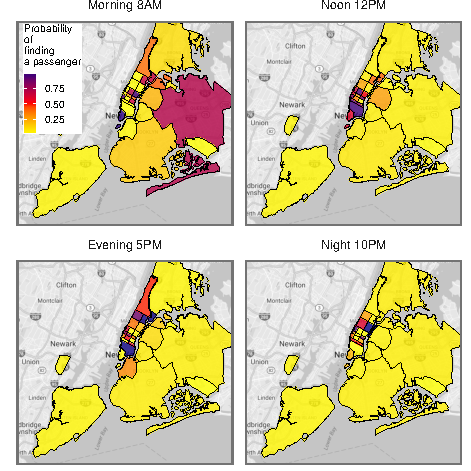
\includegraphics{figures/successful_heatmap.pdf}
	\caption{Probability of finding a passenger in 10 minutes across NYC zones at different times of the day.}
	\label{fig:successful_heatmap}
\end{figure}

Similarly, travel time matrix $\traveltimematrix^t$ and rewards matrix $\rewardsmatrix^t$ entries contain the average travel times and average rewards of traveling between two zones. Note that each entry of the {\rewardsmatrix} matrix represents net reward, calculated after taking into account the surge information, along with driver expenses and Uber's share of earnings.

Now, we describe the formation of the empirical transition matrix $\empiricaltransitionmatrix^t$. Every diagonal entry of the count matrix $\countmatrix^t$ is zero, as there are no passenger rides within same zone. However, the empirical transition matrix $\empiricaltransitionmatrix^t$ described in Section \ref{sec:problem_setup} assumes that the diagonal entries $f(i,i)$ denote the probabilities of a driver not finding a passenger in zone $i$ in the time-slice $t$. Hence, to form the empirical transition matrix, we first normalize the observed count matrix such that each of its rows sum up to 1 and call this matrix $\countmatrix^\prime$. 
In the following section, we describe the formation of empirical transition matrix $\empiricaltransitionmatrix^t$, using the matrix $\countmatrix^\prime$.

%\spara{Modeling successful passenger pickup}:
Let $N(\passengerarrivalrate)$ and $N(\driverarrivalrate)$ denote the number of passenger and driver arrivals in zone $i$ in one time unit, with Poisson arrival rates {\passengerarrivalrate} and {\driverarrivalrate} respectively. Assuming that passenger and driver arrivals are independent Poisson processes, the random variable $K = N(\passengerarrivalrate) - N(\driverarrivalrate)$ follows a Skellam distribution 
%and can be depicted by states of a Markov Chain 
such that:
\begin{equation}
\Pr[K=k] = e^{-(\passengerarrivalrate + \driverarrivalrate)} \bigg(\frac{\passengerarrivalrate}{\driverarrivalrate}\bigg) I_k\big(2 \sqrt{\passengerarrivalrate \driverarrivalrate}\big)
\end{equation}
where $I_k(z)$ is the modified Bessel function of the first kind\footnote{Although, for simplicity, we assume the independence of the passenger and driver arrival processes, we can also accommodate correlated processes with slight modification.}.

% in Figure \ref{fig:skellam_markov_chain}.


% \begin{figure}
% \begin{center}
% \begin{tikzpicture}[->, >=stealth', auto, semithick, node distance=2cm]
% \tikzstyle{every state}=[fill=white,draw=black,thick,text=black,scale=0.65]
% \node[state]    (-inf)               {$\bf ...$};
% \node[state]    (-2)[right of=-inf]   {$\bf -2$};
% \node[state]    (-1)[right of=-2]   {$\bf -1$};
% \node[state]    (0)[right of=-1]   {$\bf 0$};
% \node[state]    (+1)[right of=0]   {$\bf 1$};
% \node[state]    (+2)[right of=+1]   {$\bf 2$};
% \node[state]    (+inf) [right of=+2] {$\bf ...$};
% \path
% (-inf)  edge[bend left]         node{$\passengerarrivalrate$}   (-2)
% (-2)    edge[bend left]         node{$\passengerarrivalrate$}   (-1)
%         edge[bend left,below]   node{$\driverarrivalrate$}       (-inf)
% (-1)    edge[bend left]         node{$\passengerarrivalrate$}   (0)
%         edge[bend left,below]   node{$\driverarrivalrate$}       (-2)
% (0)     edge[bend left]         node{$\passengerarrivalrate$}   (+1)
%         edge[bend left,below]   node{$\driverarrivalrate$}       (-1)
% (+1)    edge[bend left]         node{$\passengerarrivalrate$}   (+2)
%         edge[bend left,below]   node{$\driverarrivalrate$}       (0)
% (+2)     edge[bend left]        node{$\passengerarrivalrate$}   (+inf)
%         edge[bend left,below]   node{$\driverarrivalrate$}       (+1)
% (+inf)  edge[bend left,below]   node{$\driverarrivalrate$}       (+2);
% \end{tikzpicture}
% \caption{Markov Chain depiction of Skellam Distribution}
% \label{fig:skellam_markov_chain}
% \end{center}
% \end{figure}

Whenever %the Markov Chain is in a non-positive state, 
$K<0$, there are more drivers than passengers in a given zone. We assume the worst case scenario in which a driver joins the corresponding FIFO queue at the last spot. Hence, for a state $k \leq 0$, the driver has to wait for $(|k| + 1)$ passenger arrivals in a unit time for a successful passenger pickup. The probability of a successful passenger pickup can be expressed as,
\begin{equation}
\Pr[N(\passengerarrivalrate) = |k| + 1] = \frac{\passengerarrivalrate^{\big(|k|+1\big)} e^{-\passengerarrivalrate}}{\big(|k| + 1\big)!}
\end{equation}
Thus, we can express a diagonal entry $f(i,i)$ of empirical transition matrix as follows,
\begin{equation}
f(i,i) = 1 - \sum_{k \leq 0} \Pr[K = k] \times \Pr[N(\passengerarrivalrate) \geq |k| + 1]
\end{equation}
To maintain the right stochasticity of {\empiricaltransitionmatrix}, every other entry $f(i,j)$ is calculated as,
\begin{equation}
f(i,j) = (1 - f(i,i)) \times c^\prime(i,j)
\end{equation}
The matrix $\empiricaltransitionmatrix^t$, built in this manner satisfies all our assumptions and can be used in the evaluation of strategies described in previous sections. 

Figure \ref{fig:successful_heatmap} shows an example of varying probabilities of successful pickups in different zones at various times of the day. As expected, we see that the probability of a successful pickup is higher outside Manhattan in the morning, and this trend reverses in the evening.

\begin{figure*}
	\centering
	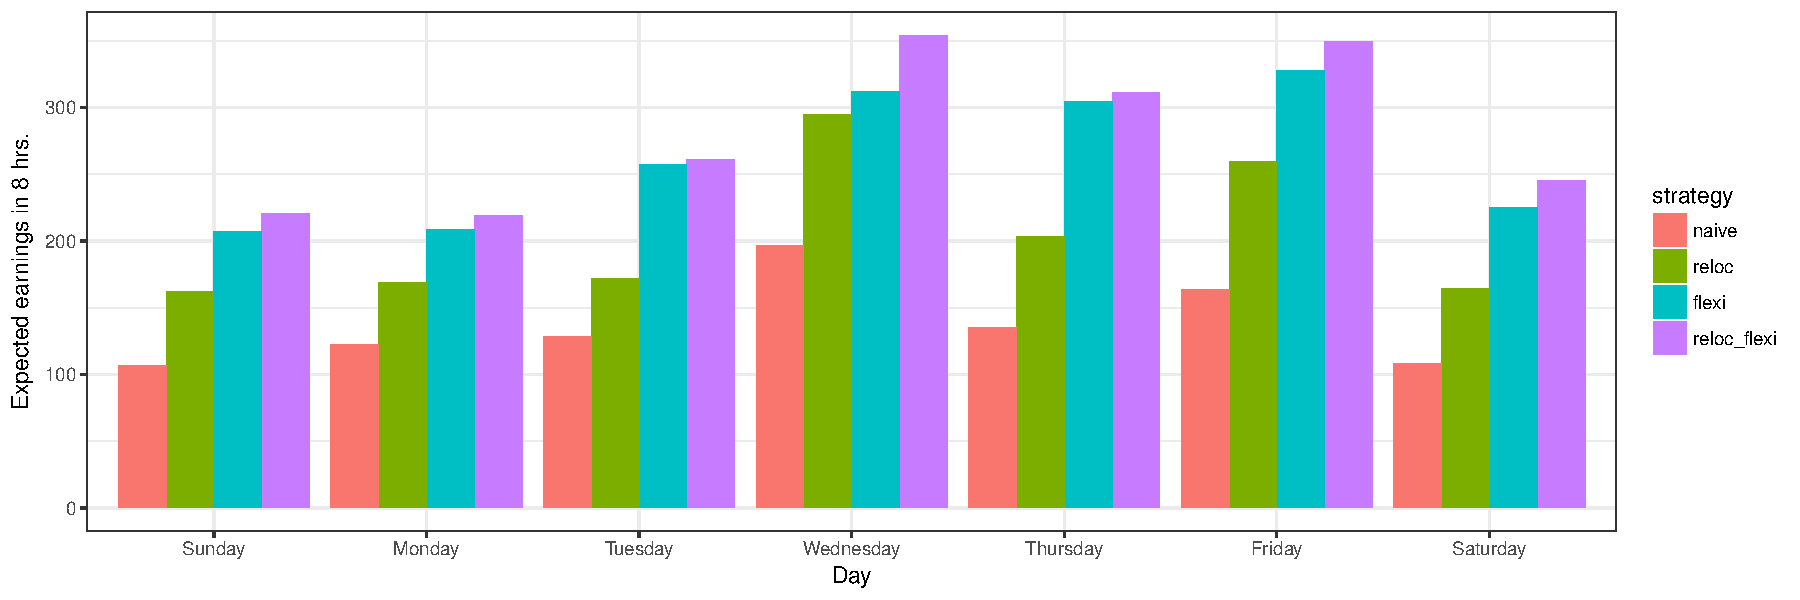
\includegraphics{figures/daily_earnings.pdf}
	\caption{Daily earnings with different strategies}
	\label{fig:daily_earnings}
\end{figure*}

\subsection{Experiments}
Now, we use the experimental framework from the previous section to evaluate various driver strategies formulated in Section \ref{sec:driver_strategies}.

\spara{Comparison of strategies}: First, we answer the question: \textit{what is the best driver strategy?} Intuitively, it is clear that {\relocationflexible} strategy is the best strategy as it takes advantage of spatial as well as temporal variations in the passenger demand across NYC. In order to verify this intuition, we compare driver earnings across different strategies. Drivers following the {\naive} and the {\relocation} strategies are assumed to drive from 9AM to 5PM, an 8 hour work day, while those following the {\flexible} or the {\relocationflexible} strategies drive for 8 hours each day with a flexible schedule.

Figure \ref{fig:daily_earnings} plots the solution to the {\originalproblem} for each of the strategies on different days of the week. For each of the day, We observe that driver earnings from {\relocationflexible} strategy are more than twice of those from {\naive}. The {\flexible} strategy always provides better earnings than even a {\relocation} strategy in 9 to 5 work schedule. Furthermore, we also observe that midweek earnings from all strategies exceed those on weekends.

\spara{Spatial dynamics of strategies}: Here, we explore the question - \textit{what are the benefits of the relocation action?} Figure \ref{fig:demand_heatmap} already shows the spatial variation in the demand across different NYC zones at different times of the day. Intuitively, this spatial variation can cause a disparity in the driver earnings based upon the zone of the driver. The {\relocation} strategy tries to reduce this disparity by allowing a driver to relocate while in a zone of low demand. To test our hypothesis, we calculate earnings from the {\naive} and the {\relocation} strategy from 8 hours of driving starting from every zone in the city, at different times of the day. We depict these earnings in form of a heatmap in Figure \ref{fig:earnings_heatmap}.

\begin{figure}
	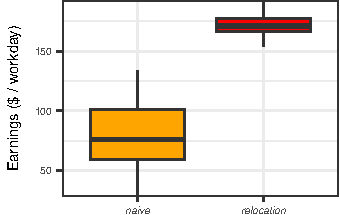
\includegraphics{figures/earnings_heatmap.pdf}
	\caption{Disparity of earnings between {\naive} and {\relocation} strategies}
	\label{fig:earnings_heatmap}
\end{figure}

We observe that, as expected, the variation in the {\naive} strategy earnings is substantial at all times of the day. Most notably, in the morning hours, drivers from zones surrounding Manhattan and those from near JFK airport earn considerably more than others. The {\relocation} strategy balances out this variation in earnings to some extent, while consistently outperforming the {\naive} strategy across all zones.

\spara{Temporal dynamics of strategies}: It is obvious from Figure \ref{fig:daily_earnings} that both of the flexible schedule strategies outperform their fixed schedule counterparts. So, we explore the question \textit{what is the best time of the day to drive in order to maximize earnings?} As the choice of the {\gohome} action depends on multiple factors such as the location of the driver, the demand across the city, the budget left, etc., we visualize preferred driving hours using 1000 simulated drivers. Each driver has a randomly assigned home zone. At every step throughout the day, simulated drivers follow actions recommended by the contingency plans developed while solving the {\originalproblem} for {\flexible} and {\relocationflexible} strategies.

\begin{figure}[H]
	\centering
	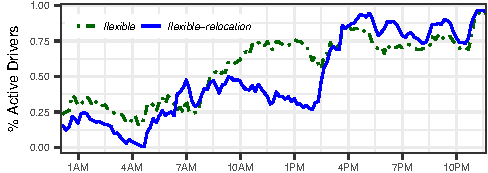
\includegraphics{figures/simulated_schedules.pdf}
	\caption{Active drivers with {\flexible} and {\relocationflexible}
	strategies at different times of the day.}
	\label{fig:simulated_schedules}
\end{figure}

We observe that drivers of both {\flexible} and {\relocationflexible} strategies are active in large percentages after 7PM in the evening. However, over 50\% of the drivers following the {\flexible} strategy are active throughout the day after 8AM in the morning. In stark contrast with them, drivers following the {\relocationflexible} strategy are active in overwhelming percentages during peak hours of the day, from 6AM to 10AM in the morning, and post 7PM in the evening. This makes us conclude that {\relocate} action is more effective during the peak hours, thereby prompting higher percentages of {\relocationflexible} drivers to be active in those hours.

\spara{Preferred relocation zones}:
Simulated drivers also allow us to compare the {\relocate} actions between drivers following {\relocation} strategy and those following {\relocationflexible} strategy. The endzones for relocate actions of drivers are shown in Figure \ref{fig:relocation_endzones}. We observe a contrast between the preferred relocation zones for drivers of either strategies. Drivers following the {\relocation} strategy predominantly relocate themselves to zones `3A', `3C', `4A' zones near the West Village neighborhood and zones `7B' and `8' near the LaGuardia Airport, while those following the {\relocationflexible} strategy relocate themselves to zone `1' comprising of the Financial District and zones `5A', `5B' and `6B' near the Upper East side of New York City.

\begin{figure*}
	\centering
	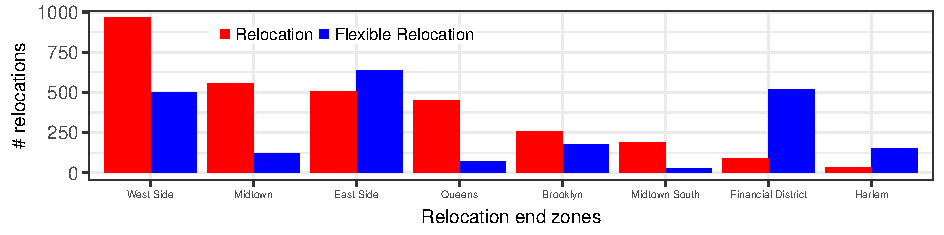
\includegraphics{figures/relocation_endzones.pdf}
	\caption{Contrast between preferred relocation endzones for drivers with 
	{\relocation} and {\relocationflexible} strategies}
	\label{fig:relocation_endzones}
\end{figure*}

\subsection{Surge Chasing}
\begin{figure}[H]
	\centering
	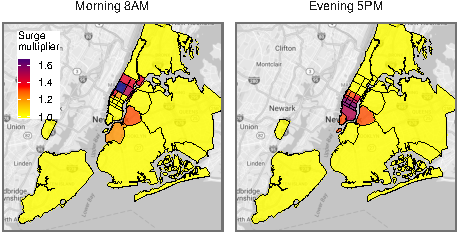
\includegraphics{figures/surge_heatmap.pdf}
	\caption{Active surge multiplier across NYC zones at different times of the day.}
	\label{fig:surge_heatmap}
\end{figure}
Now that we have an understanding about the various driver strategies, we turn our attention to surge pricing. Surge pricing is a controversial feature of the Uber platform. According to Uber, it encourages drivers to start driving during the peak hours in order to efficiently meet demand with supply, albeit at a higher cost to passenger, in turn leading to higher driver earnings. In fact, Uber prominently displays to drivers on their Partner App, the information regarding surge multiplier in different geographical neighborhoods in form of a heatmap. However, as the Uber's surge pricing algorithm is proprietary, it is unclear whether drivers should relocate themselves to surging areas consistently in order to maximize their earnings. Using our information about surge multipliers, we are in a position to answer the question-- \textit{Should drivers engage in surge chasing?}
\begin{figure}[H]
	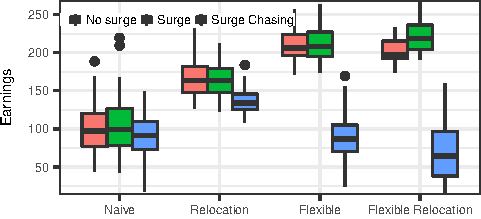
\includegraphics{figures/simulated_earnings.pdf}
	\caption{Simulated earnings for drivers across different strategies.}
	\label{fig:simulated_earnings}
\end{figure}
In order to do so, we evaluate earnings of simulated drivers in three scenarios viz., `no surge' - where we disable the surge multiplier, `surge' - where surge multiplier is accounted for while calculating earnings, and `surge chasing' wherein surge multiplier is enabled and a driver `chases surge' i.e, a driver located in a non-surging zone always relocates to the zone with highest surge multiplier. The earnings of the simulated drivers in these scenarios are shown in Fig. {\ref{fig:simulated_earnings}}. We observe that `chasing surge' in {\naive} strategy on an average yields slightly less earnings than even the situation when surge multiplier is disabled. Interestingly, chasing surge is even more ill-advised if the driver follows a flexible schedule strategy, and it can lead to huge losses.

\subsection{Effect of uncertainty} 

All the experiments described in previous section indicate that our strategies always outperform a {\naive} strategy most prevalent among the drivers. However, it is worth noting that our strategies are evaluated based on historical data. Consequently, such strategies can be highly sensitive to changes in the underlying data, in form of perturbed transition matrices. We can recommend our strategies to drivers only if they outperform the {\naive} strategy in presence of such perturbations. Hence, using the framework developed in Section \ref{sec:sensitivity}, we solve the {\robustproblem} problem for each of the four strategies for increasing levels of uncertainty in the transition matrices.

Figure \ref{fig:uncertainty_evolution} shows the results of increasing uncertainty on the earnings of drivers following each of the four strategies. Not only are the {\relocation}, {\flexible} and {\relocationflexible} strategies more tolerant to uncertainty in transition matrices, but they outperform the {\naive} strategy at 0\% uncertainty, while themselves at with 99\% uncertainty. This provides evidence regarding the robustness of such strategies.

\begin{figure}[H]
	\centering
	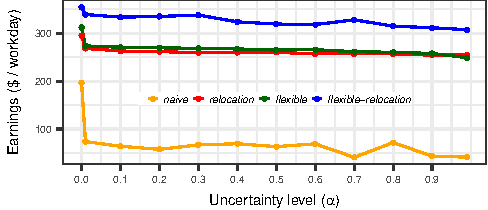
\includegraphics{figures/uncertainty_evolution.pdf}
	\caption{Sensitivity to uncertainty in parameters.}
	\label{fig:uncertainty_evolution}
\end{figure}

% \subsection{\textsc{RewardsMatrix}}

% The data gathered in the previous section gives us a matrix of driver earnings, \matr{E}, from passengers while traveling between any two zones in the city. We also get a costs matrix, \matr{C}, whose each entry, $c(i,j) \leq 0$, denotes the sundry expenses of traveling from zone $i$ to zone $j$, dependent on distance and traffic at the given time. The travel costs can result in negative net rewards in the {\gohome} and {\relocate} actions, violating the assumption from Section \ref{sec:problem_setup} that $r(i,j) \geq 0$. In this section, we describe the construction of \textsc{RewardsMatrix}, {\rewardsmatrix}, corresponding to each driver action compliant with our assumptions.

% \subsubsection{\textsc{Modifying the CostsMatrix}}
% If $min\_cost$ is the minimum entry in the matrix \matr{C}, each entry of the modified costs matrix, \matr{C'} is calculated as,
% \begin{equation}
% c'(i,j) = c(i,j) - min\_cost
% \end{equation}
% As a result of the above modification, $\forall i,j : c'(i,j) \geq 0$.

% \subsubsection{\textsc{RewardsMatrix}}
% In order to be compliant with the assumption in Section \ref{sec:problem_setup}, we define two kinds of \textsc{RewardsMatrix}, one for the action {\getpassenger} and another for the actions {\gohome} and {\relocate}.

% \begin{itemize}
% 	\item For the {\getpassenger} action, we define the rewards matrix as,
% 	\begin{equation}
% 		r(i,j) = e(i,j) + c'(i,j) 
% 	\end{equation}
% 	\item For the {\gohome} and {\relocate} actions, the rewards matrix is same as the modified costs matrix.
% 	\begin{equation}
% 		r(i,j) = c'(i,j)
% 	\end{equation}
% \end{itemize}
% In both cases, we set the diagonal entries of the matrix to zero i.e., $\forall i: r(i,i) = 0$.

% It should be noted that this modification does not affect the optimal action choice in any strategy. It merely ensures that the input vectors to the Bisection Algorithm from Section \ref{sec:sensitivity} are always non-negative vectors. Furthermore, while calculating the actual {\totalexpectedearnings} of a driver, we can backtrack these modifications.

% \subsection{\textsc{Comparing robust and nominal strategies}}
% In this section, we compare various strategies. When we choose, $\beta = \betamax$, there is no uncertainty, and we get solution computed via the classical Bellman recursion; referred to as nominal strategy. The robust strategy corresponds to solving the MDP with varying values of $\beta$.

% \subsection{\textsc{Effect of Inaccuracy is uncertainty level}}
% The previous section assumes that, in the robust case, we are able to estimate exactly the precise value of the uncertainty level. In practice, the parameter $\beta$ also has to be estimated. In this section, we study the sensitivity of the robust approach with respect to inaccuracies in the uncertainty parameter $\beta$.
%!TEX root = main.tex

\section{Conclusions}
\label{sec:conclusions}

The challenge of how to maximize one's individual earnings as a driver for a 
ridesharing platform like Uber or Lyft is a pressing question that millions of micro-entrepreneurs 
across the world now face.  Anecdotally, many drivers spend a great deal of time 
strategizing about where and when to drive.  However, to date, drivers are either
self-taught and use heuristics of their own devising, or learn from one another.
Indeed, rumors suggest that some drivers even collude in attempts to induce spikes in surge 
prices that they can then exploit.
In this work, we confirm the power of strategic driving behavior, by simulating 
key points in the strategy space optimized against realistic data-driven projections
of ridership in the NYC area.  Our first key takeaway is that a naive driver,
armed with no data, and driving a 9-5 random walk schedule, is leaving 
roughly a 50\% hourly pay raise on the table by not driving more strategically 
in terms of time and location.  In contrast, a data-savvy driver armed with
good historical data can build a forecast and optimal contingency plans for 
an upcoming week of driving with a couple hours of computational overhead using 
our dynamic programming algorithms, with provable resilience to input
uncertainty.  Our experimental and simulation results yield insights into the
structure of highly optimized schedules, including relatively frequent relocation,
working at specific peak periods, and opportunistically taking advantage of 
surges when the time is ripe.  

An obvious limitation of our work is that it is tailored to the setting when the 
methods are employed by self-interested individuals.  If and when a 
significant percentage of the labor supply employs sophisticated optimization methods
for driving, one would need to consider different strategies that lead either to mixed 
equilibria, or achieve other global objective functions, as opposed to the simple 
greedy approach we invoke here.  Indeed, in the long run, as drivers for ridesharing 
platforms like Uber and Lyft are put out of work by fleets of autonomous vehicles, 
the formulation and solution of new sets of optimization problems along those lines
are likely to become relevant as well.





\bibliographystyle{ACM-Reference-Format}
%\bibliographystyle{ormsv080}
\bibliography{sigproc} 

\end{document}
